\section{The Mobile Application}
This project is focused on the customers of Software Development companies and how we can ease the communication between the customers and the companies.
Therefore we will create a Mobile Application for the customers that should act as a hub for the customer. 
This application should allow the customer to follow along with the progress of the development alongside allowing the customers to specify requirements for the system under development in an intuitive "What You See Is What You Get" (WYSIWYG) environment.

We envision the application to have the following features:

\begin{itemize}
    \item A KanBan inspired board of all issues/ tasks throughout the lifespan of the development
    \item The ability to show the developer comments on any issue/ task and show all Git branches related to an issue or task
    \item A WYSIWYG editor for creating requirements for the visuals of the system under development
    \item A module for running all the tests on the current master build of the system such that the customer can see how many requirements are currently fulfilled
    \item A module inside the WYSIWYG editor for specifying the behavior of the system, such as, when this text field is left empty shows an error message
    \item A repository for creating and managing actors of the system under development
    \item A repository for creating and managing data entities of the system
\end{itemize}

During the discovering phase of ideas for the Mobile Application, we created a set of rough prototypes in the form of drawings, we will now present these drawings as a measure for more clearly illustrate our vision.

\begin{figure}[H]
    \centering
        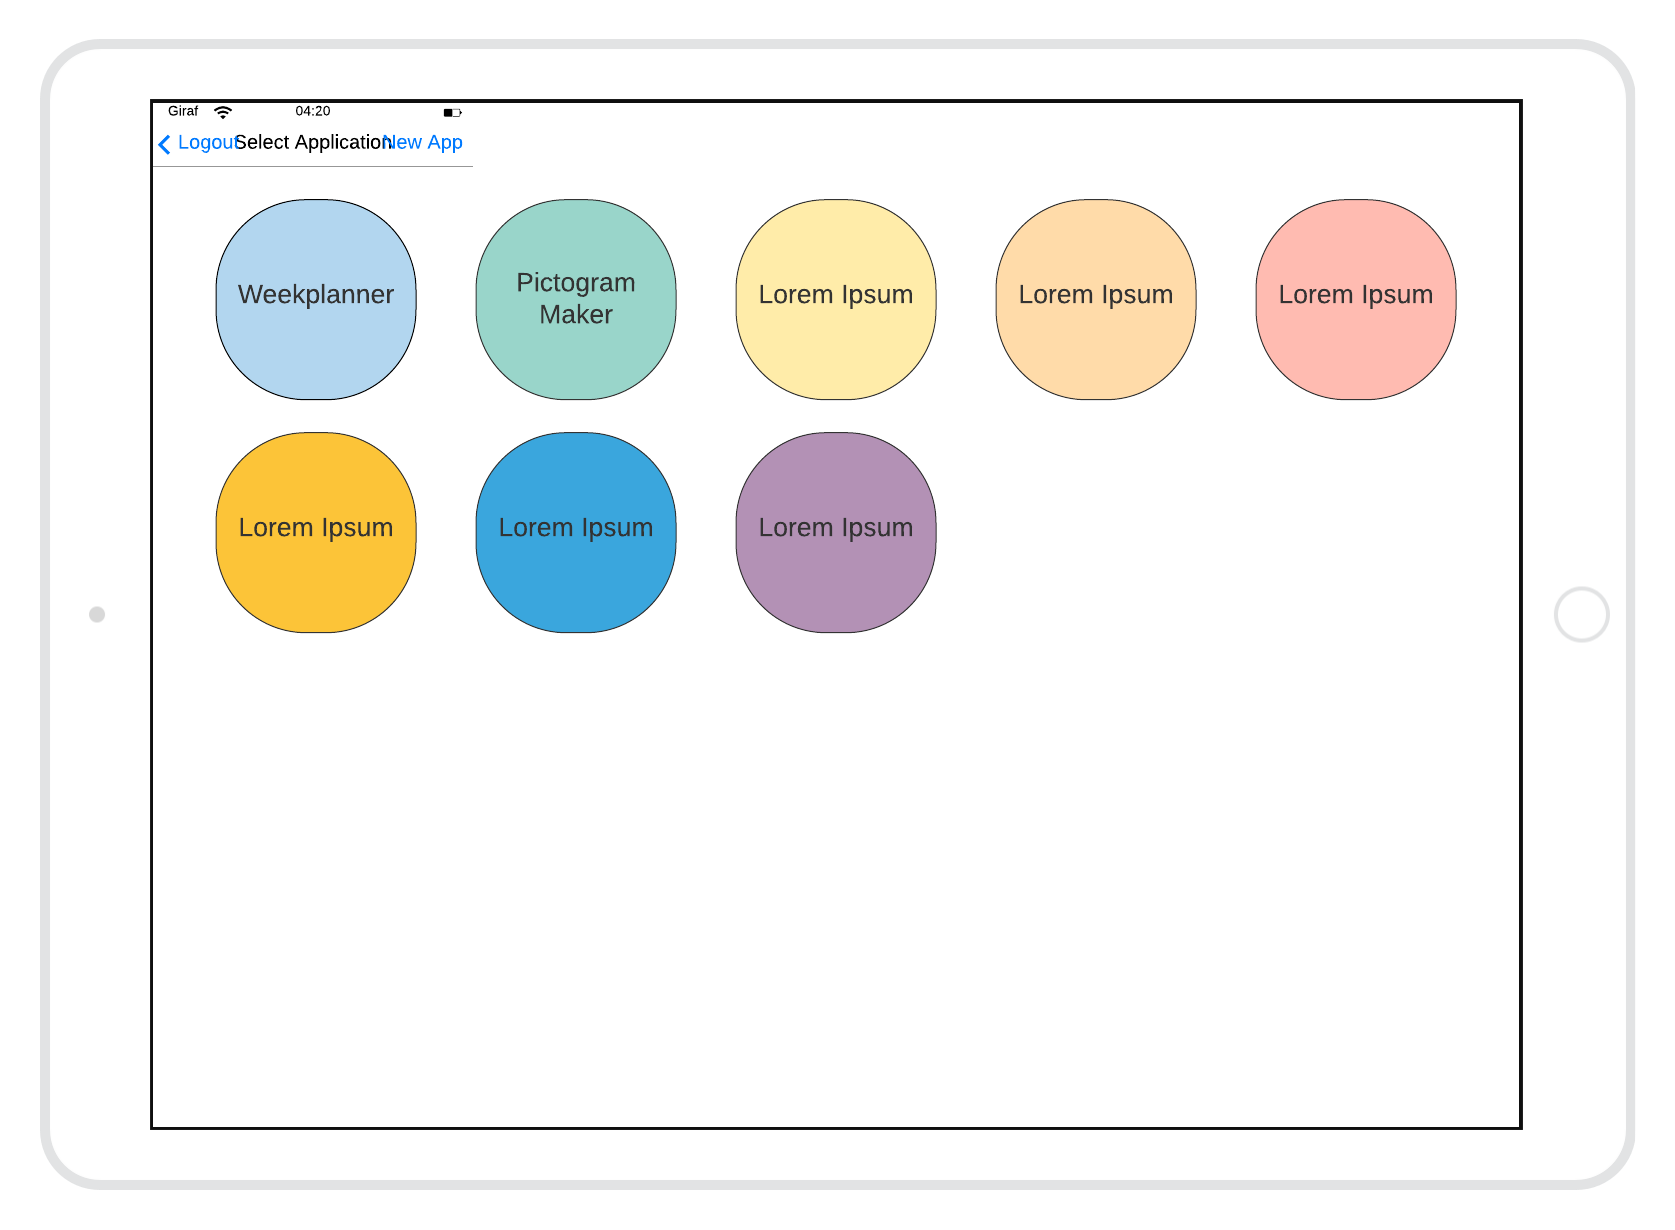
\includegraphics[width=\textwidth]{images/Select-App-Mockup.png}
        \caption{Prototype of Select Development project.}
\end{figure}
\begin{figure}[H]
    \centering
    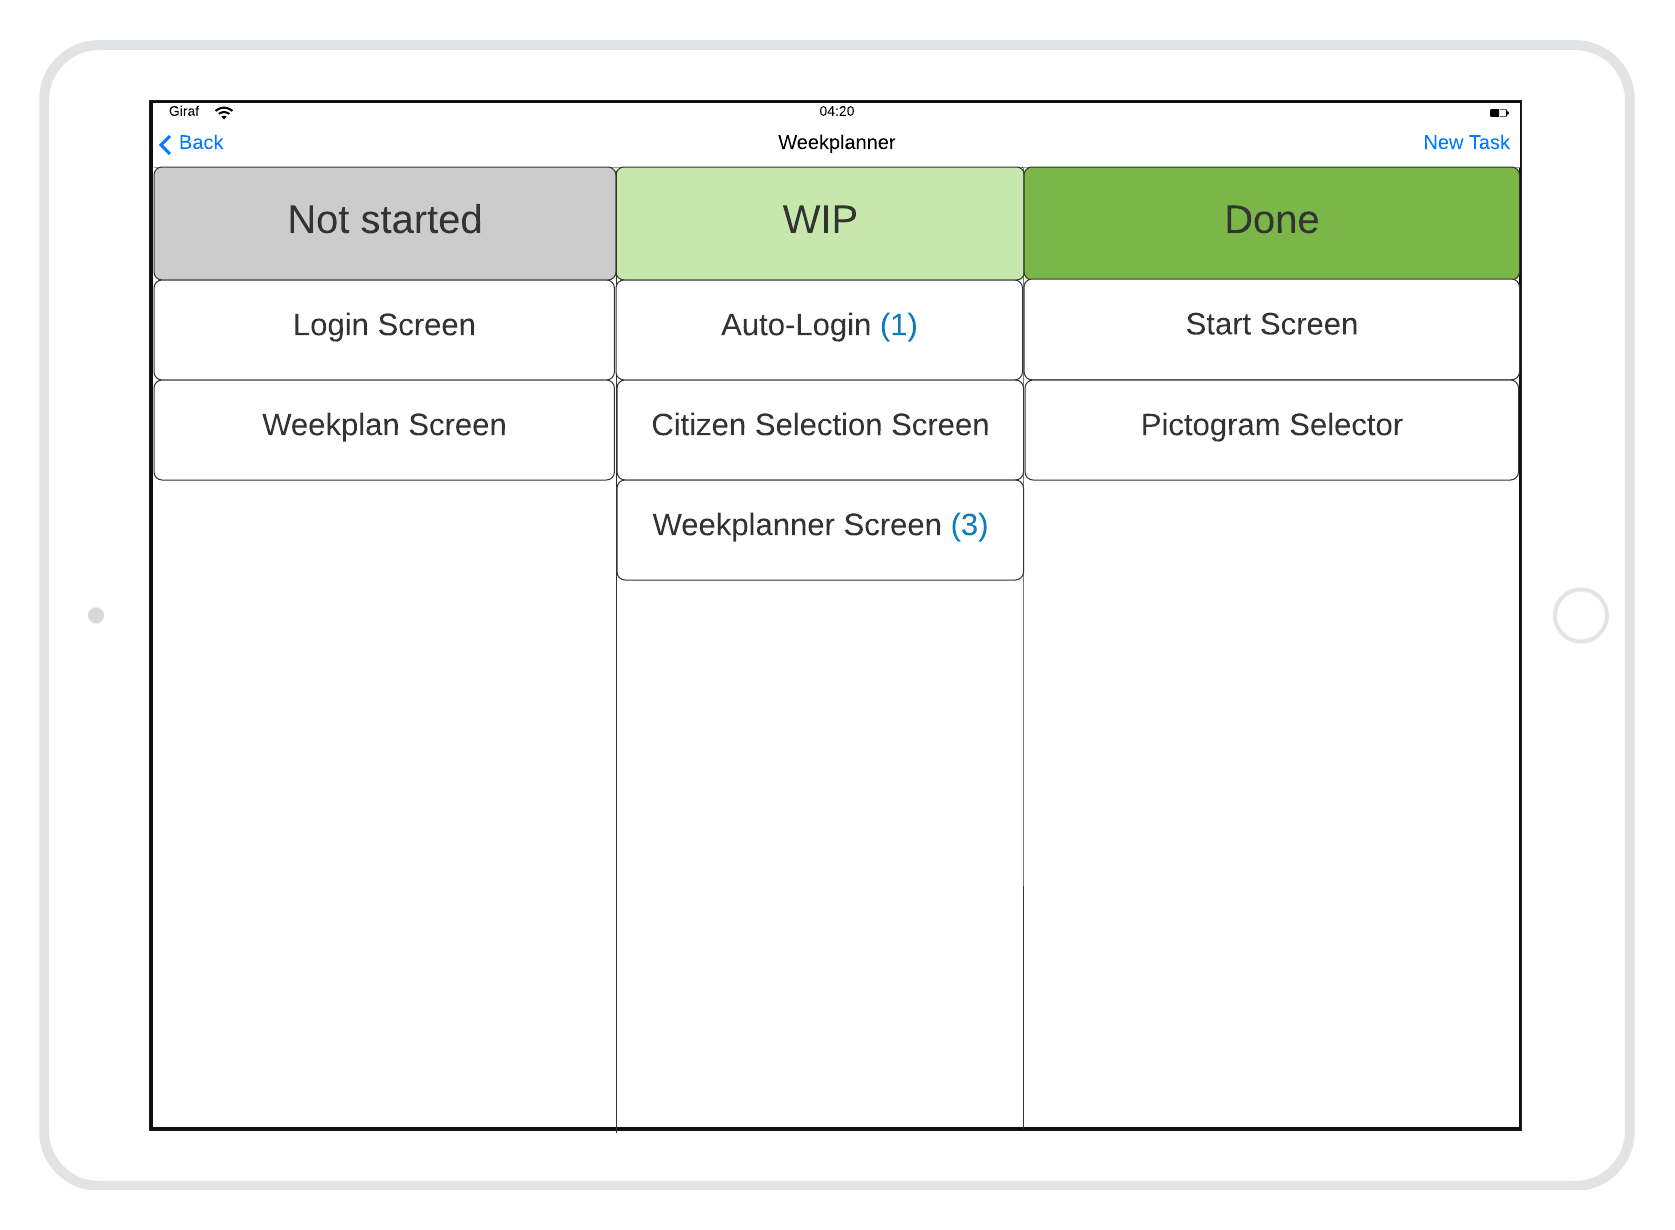
\includegraphics[width=\textwidth]{images/KanBan-mockup.png}
    \caption{Prototype of KanBan Board for a perticular development project.}
\end{figure}
\begin{figure}[H]
    \centering
    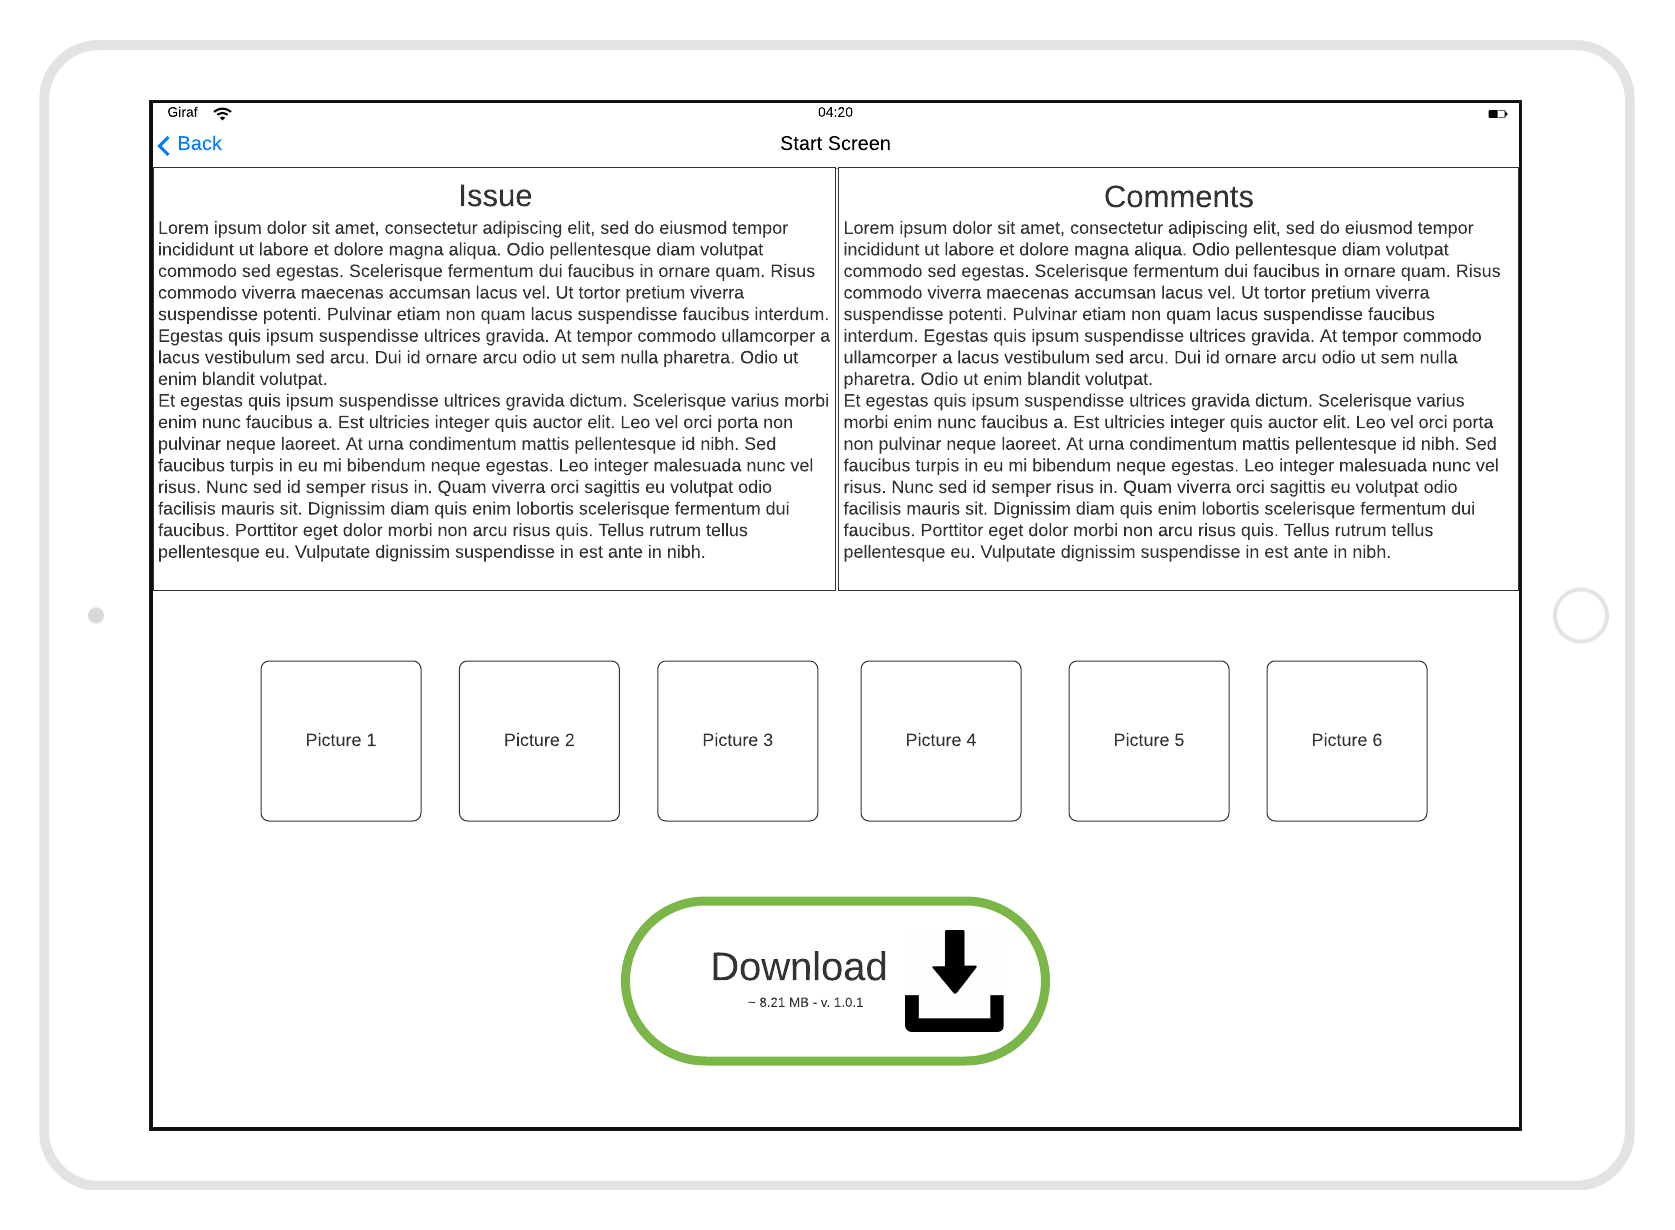
\includegraphics[width=\textwidth]{images/view-a-task-mockup.png}
    \caption{Prototype of status of a singular task.}
    \label{FIG:mockupIssuesComments}
\end{figure}